\documentclass[a4paper,kulak]{kulakarticle}

\usepackage[utf8]{inputenc}
\usepackage[dutch]{babel}
\usepackage[]{amsmath}
\usepackage{float}
\usepackage{subcaption}
\usepackage{graphicx,wrapfig,lipsum}

\date{Academiejaar 2018-2019}
\address{
  Informatica \\
  Statistische modellen en data-analyse \\
  Prof. Stefan Van Aelst \& Stijn Rebry}
\title{Verslag project 1}
\author{Thomas Bamelis R0640219 \& Michiel Jonckheere R0665594}

\begin{document}

\maketitle

\tableofcontents
\newpage
\section*{Introductie}
In dit verslag wordt nagegaan hoe de oorzaken van overlijden verschillen tussen landen en regio's in
de wereld. Er zijn schattingen van het aantal overlijdens beschikbaar voor 183 landen,
opgesplitst naar 32 verschillende doodsoorzaken. De landen worden gegroepeerd in 6 groepen volgens
geografische ligging en 2 groepen naargelang de globale ontwikkeling van het betreffende land. De gegevens
met betrekking tot de doodsoorzaken zijn afkomstig van de Wereldgezondheidsorganisatie \cite{ghe} en betreffen
het jaar 2016, de indeling in groepen is deze volgens de Verenigde Naties \cite{vn}. 

\section{Clustering}
Als eerste werd een cluster-analyse uitgevoerd op de gegevens. Eerst bespreken we de gegevens zonder schalen, daarna met.
\subsection{Zonder schalen}
Om een idee te krijgen van hoeveel clusters er best worden genomen, werden het agglomerate nesting algoritme en divisive analysis toegepast.
Agglomerate nesting werd gedaan met de volgende dissimilariteiten: group average, nearest neighbour en furthest neighbour, in die volgorde met daarna divisive analysis.
Zie figuren \ref{fig:hcnd} en \ref{fig:hcnb} in de bijlage \ref{b}.
Gegeven deze figuren lijkt het meest aannemelijk om 2, 4 en 6 klassen te proberen.
De gebruikte clustering algoritmes zijn in volgorde k-means, partitioning around mediods en fuzzy analysis.
De clustering ermee voor 2, 4 en 6 klassen werd geëvalueerd via een silhouette plot en een clusplot.
Zie figuur \ref{fig:cne}.
Hieruit blijkt dat partitioning around mediods met 2 clusters het beste presteert met een silhouette coëfficiënt van 0.50 (cluster 1 : 0.69 en cluster 2 : 0.43).
Dit is niet bepaald goed en balanceert op het randje van een zwakke structuur.
\subsection{Met schalen}
 We trekken hierbij dezelfde conclusies omtrent het aantal klassen, 2, 4, en 6.
 Zie figuren \ref{fig:hcd} en \ref{fig:hcb}
 Na dezelfde clustering algoritmes toegepast te hebben (figuur \ref{fig:ce}), is de best geobserveerde silhouette coëfficiënt 0.23.
 Hieruit besluiten we dat clustering met schalen aanzienlijk slechter is dan zonder schalen.
 We besluiten dus verder te werken met het beste resultaat zonder schalen.
 \subsection{Beschrijving clusters}



\section*{Besluit}

TODO


\begin{thebibliography}{9}
	
	\bibitem{ghe}
	Global Health Estimates 2016: Deaths by Cause, Age, Sex, by Country and by Region, 2000-2016.
	Geneva, World Health Organization; 2018.
	
	\bibitem{vn}
	Country classification, june 2018. Geneva, United Nations Conference on Trade and Development;
	2018.
	
\end{thebibliography}

\section{Bijlage} \label{b}
\subsection{Clustering}
\subsubsection{Zonder schalen}
\begin{figure}
	\centering
	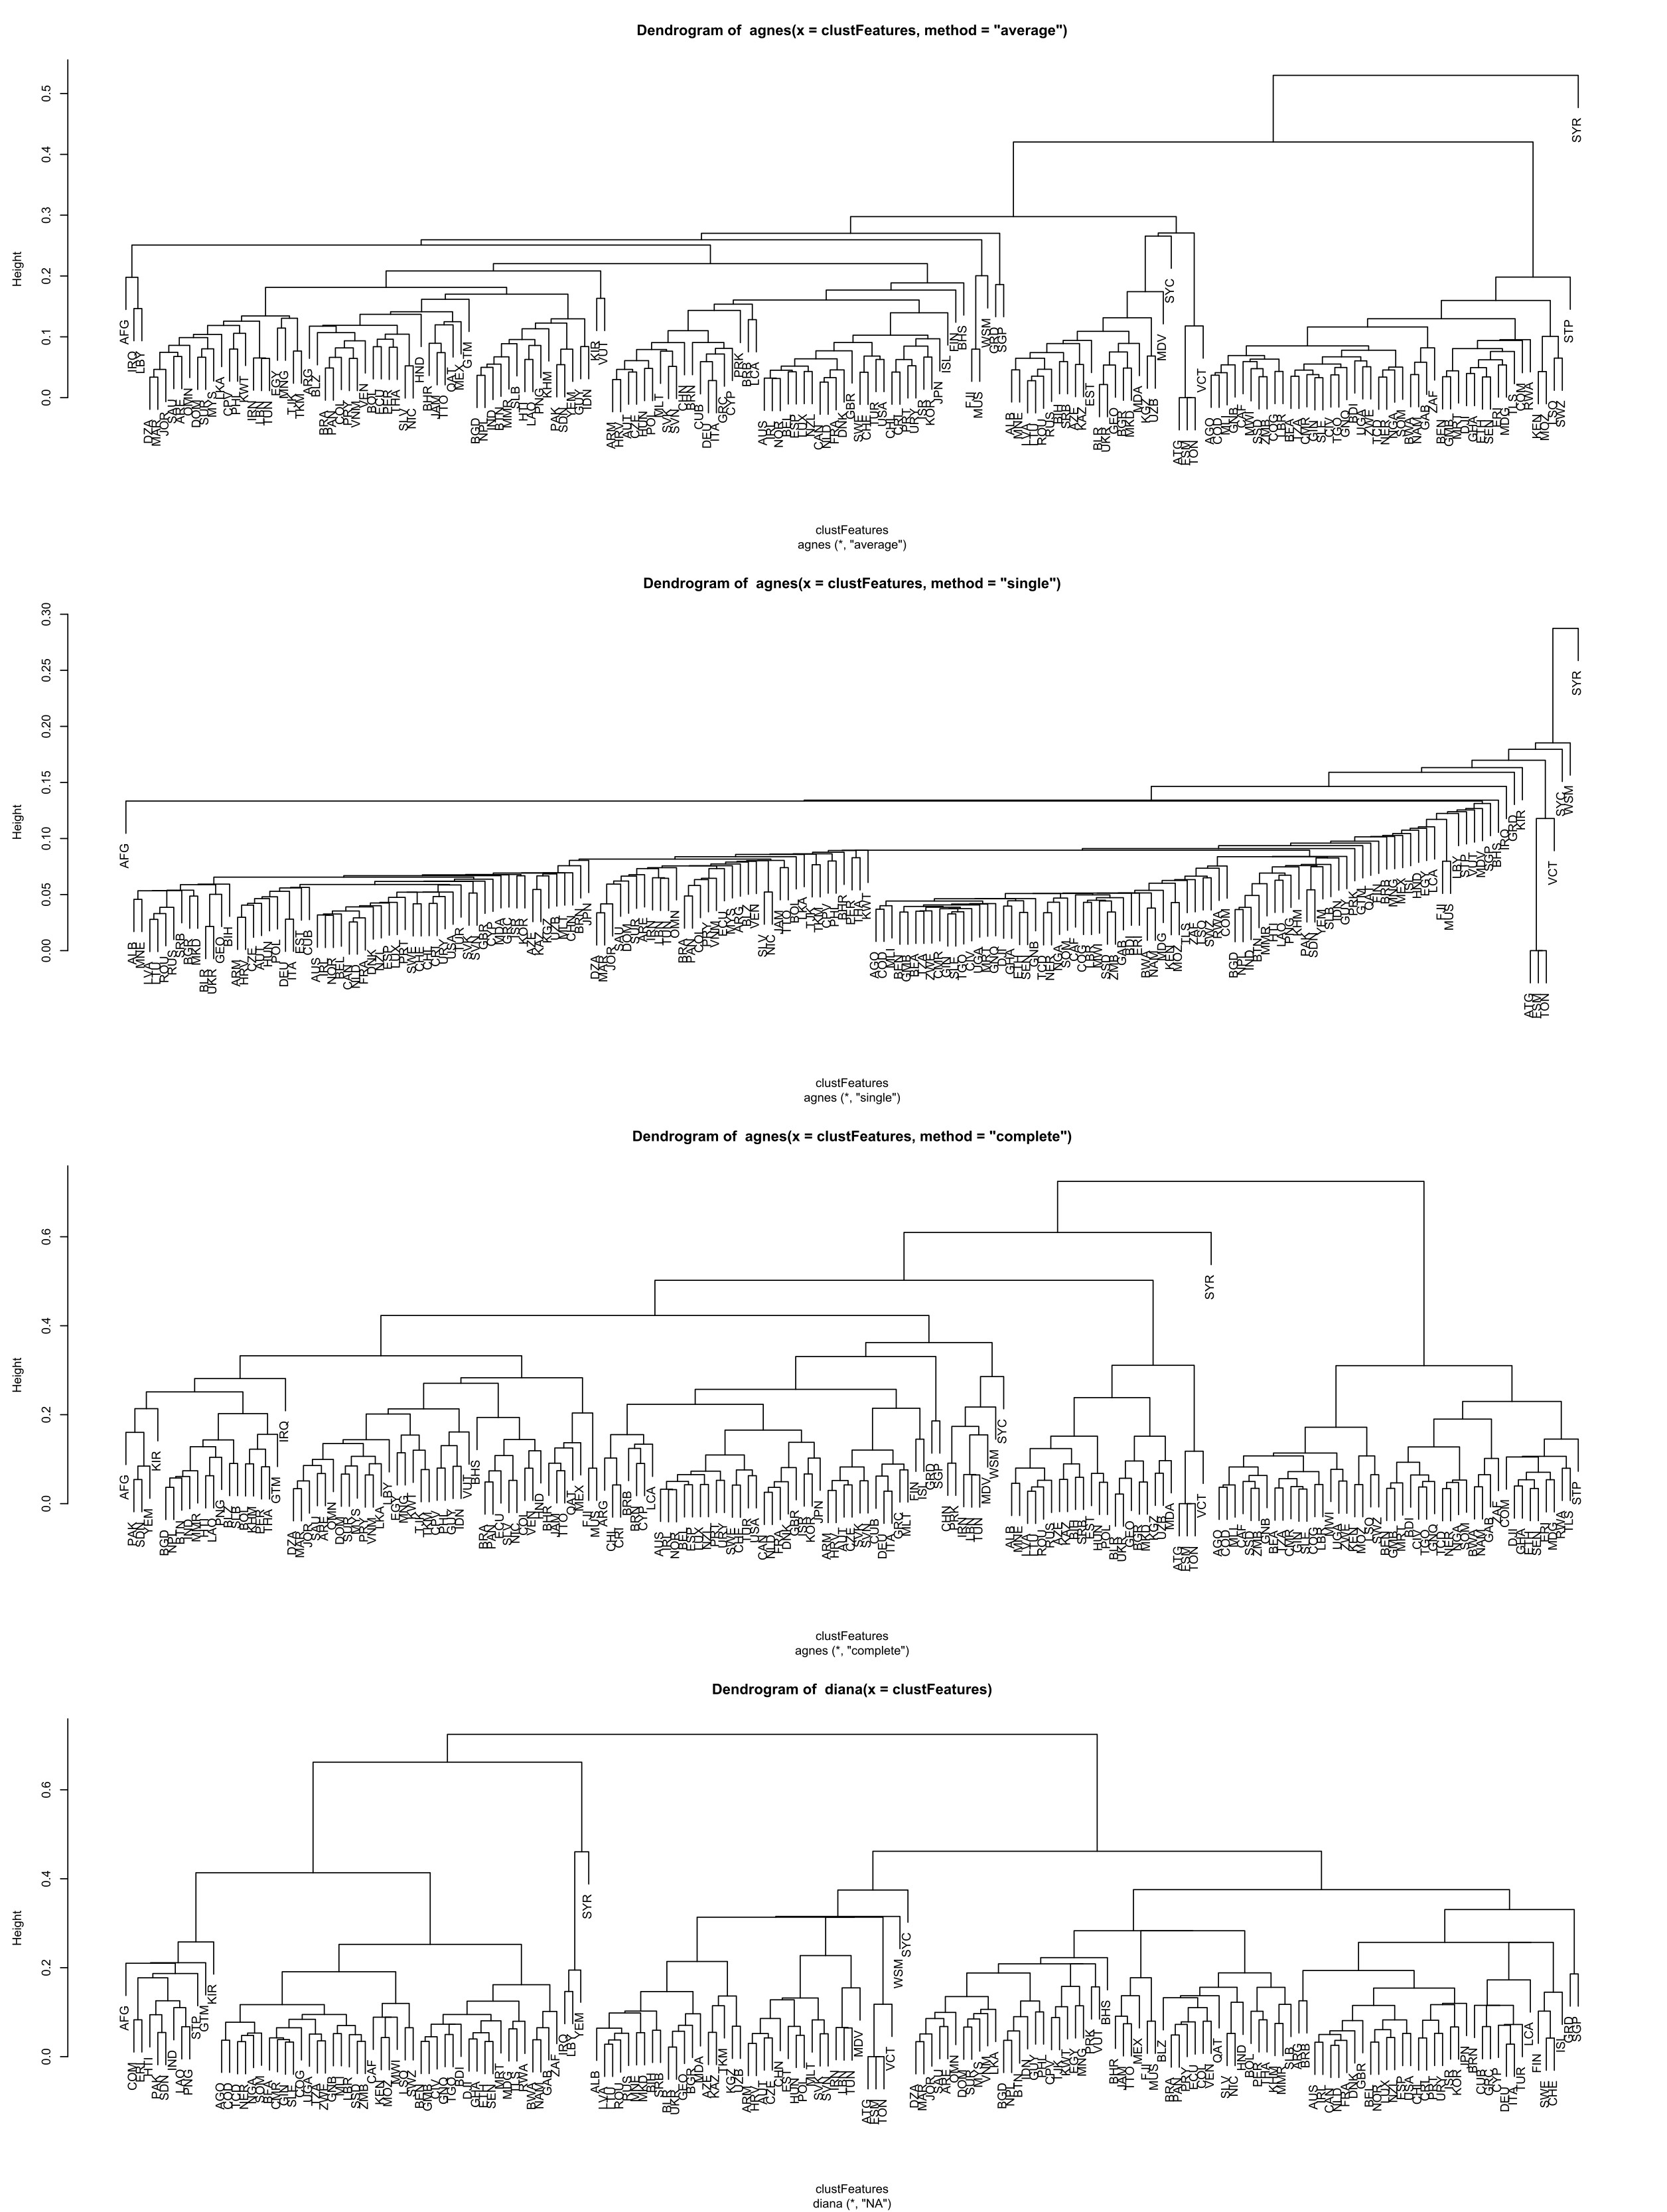
\includegraphics[height=\textheight]{figures/hierachicalClusteringNoScalingDendogram.jpg}
	\caption{Hierchical clustering dendograms}
	\label{fig:hcnd}
\end{figure}
\begin{figure}
	\centering
	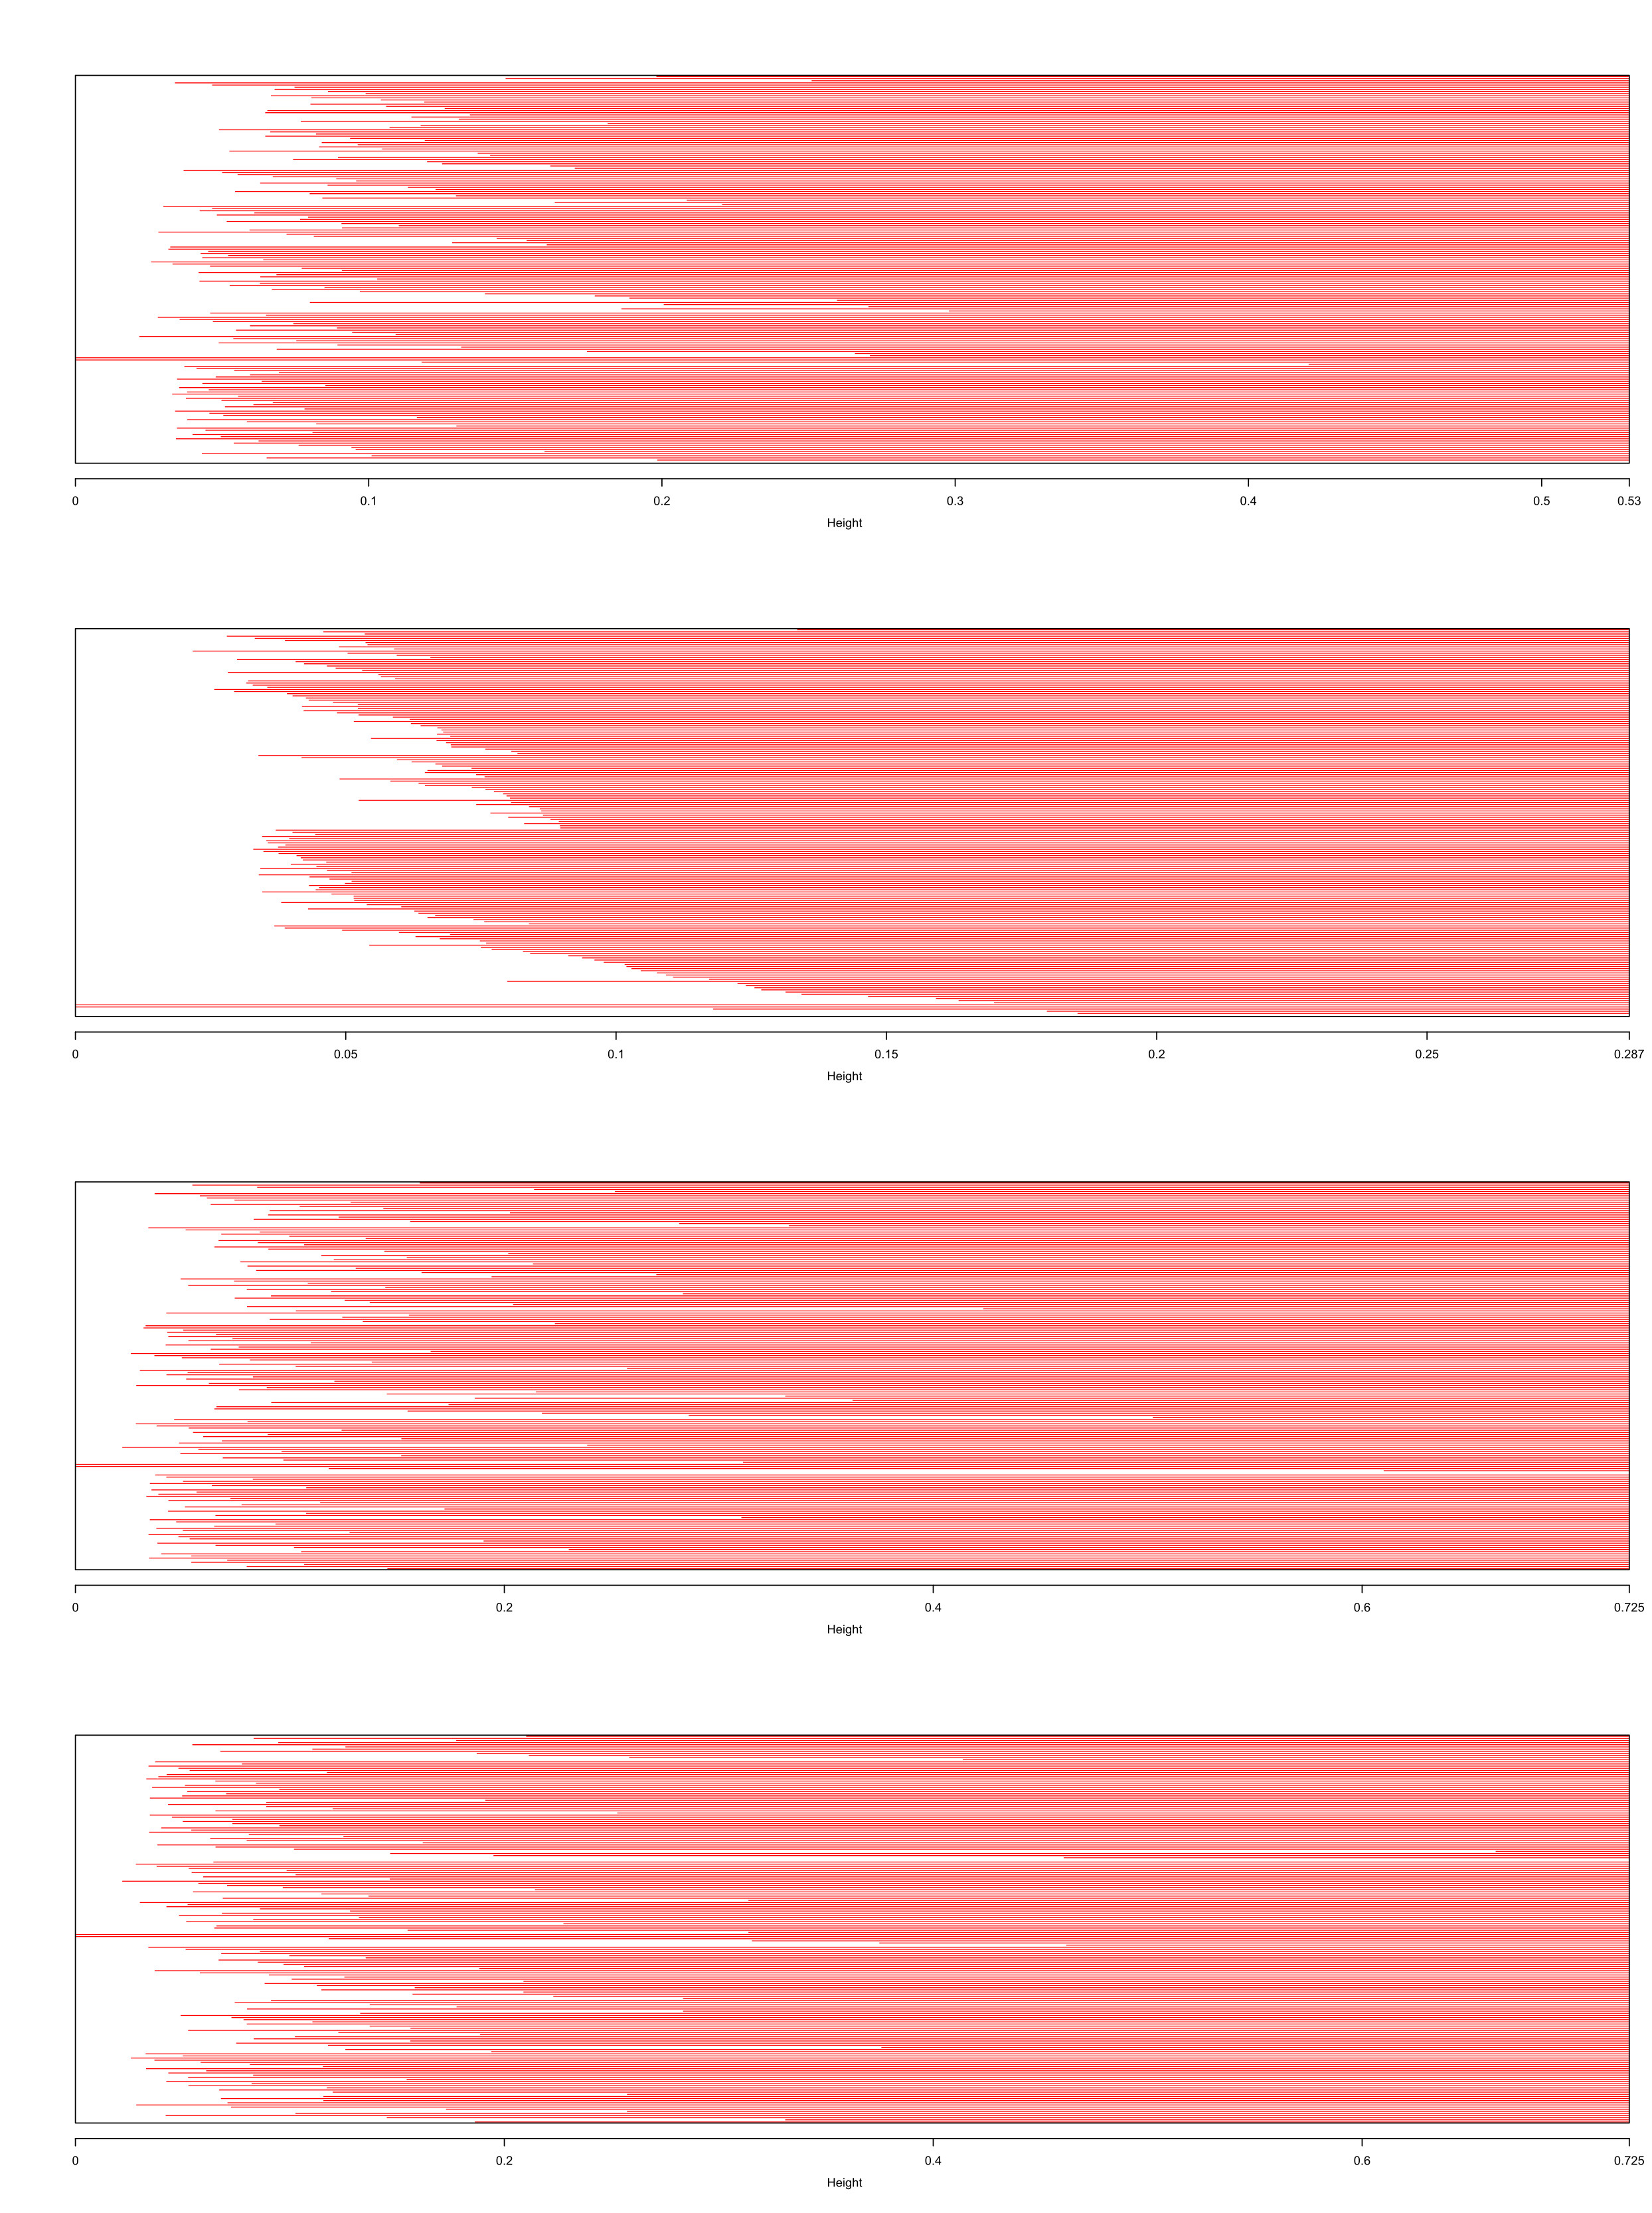
\includegraphics[height=\textheight]{figures/hierachicalClusteringNoScalingBanner.jpg}
	\caption{Hierchical clustering bannerplots}
	\label{fig:hcnb}
\end{figure}
\begin{figure}
	\centering
	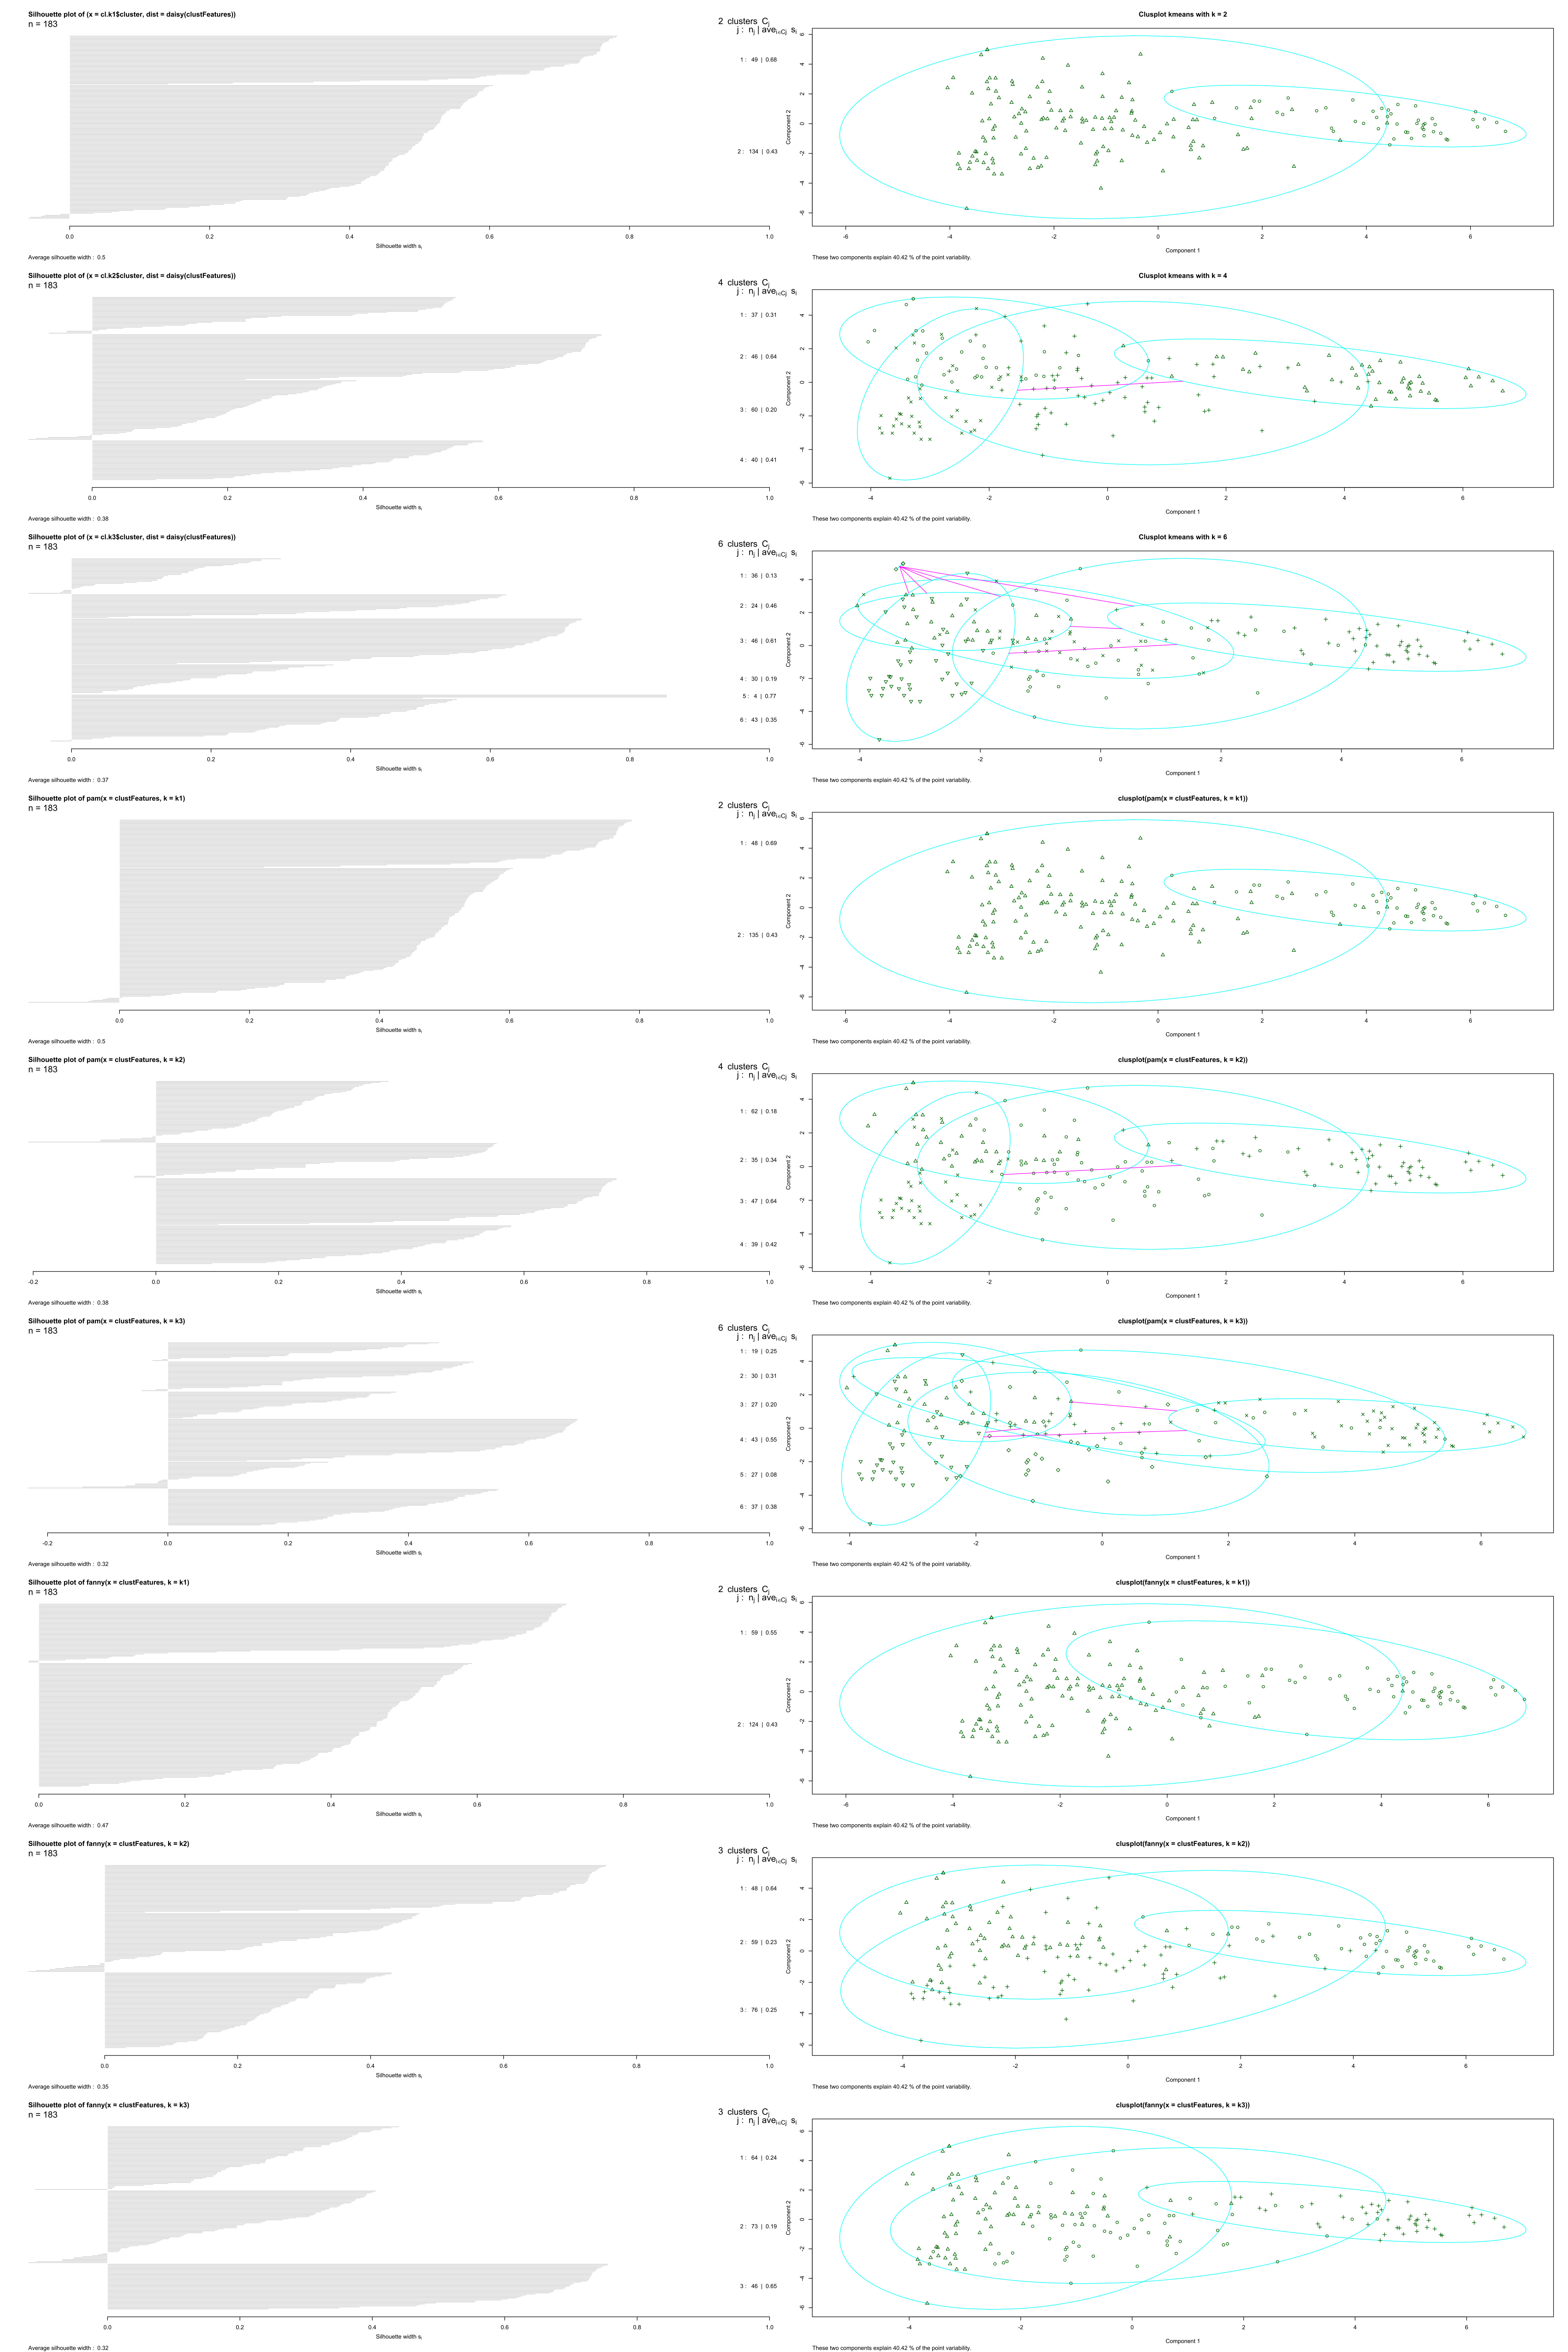
\includegraphics[height=\textheight]{figures/clusteringEvaluationNoScaling.jpg}
	\caption{Clustering evaluatie}
	\label{fig:cne}
\end{figure}
\subsubsection{Met schalen}
\begin{figure}
	\centering
	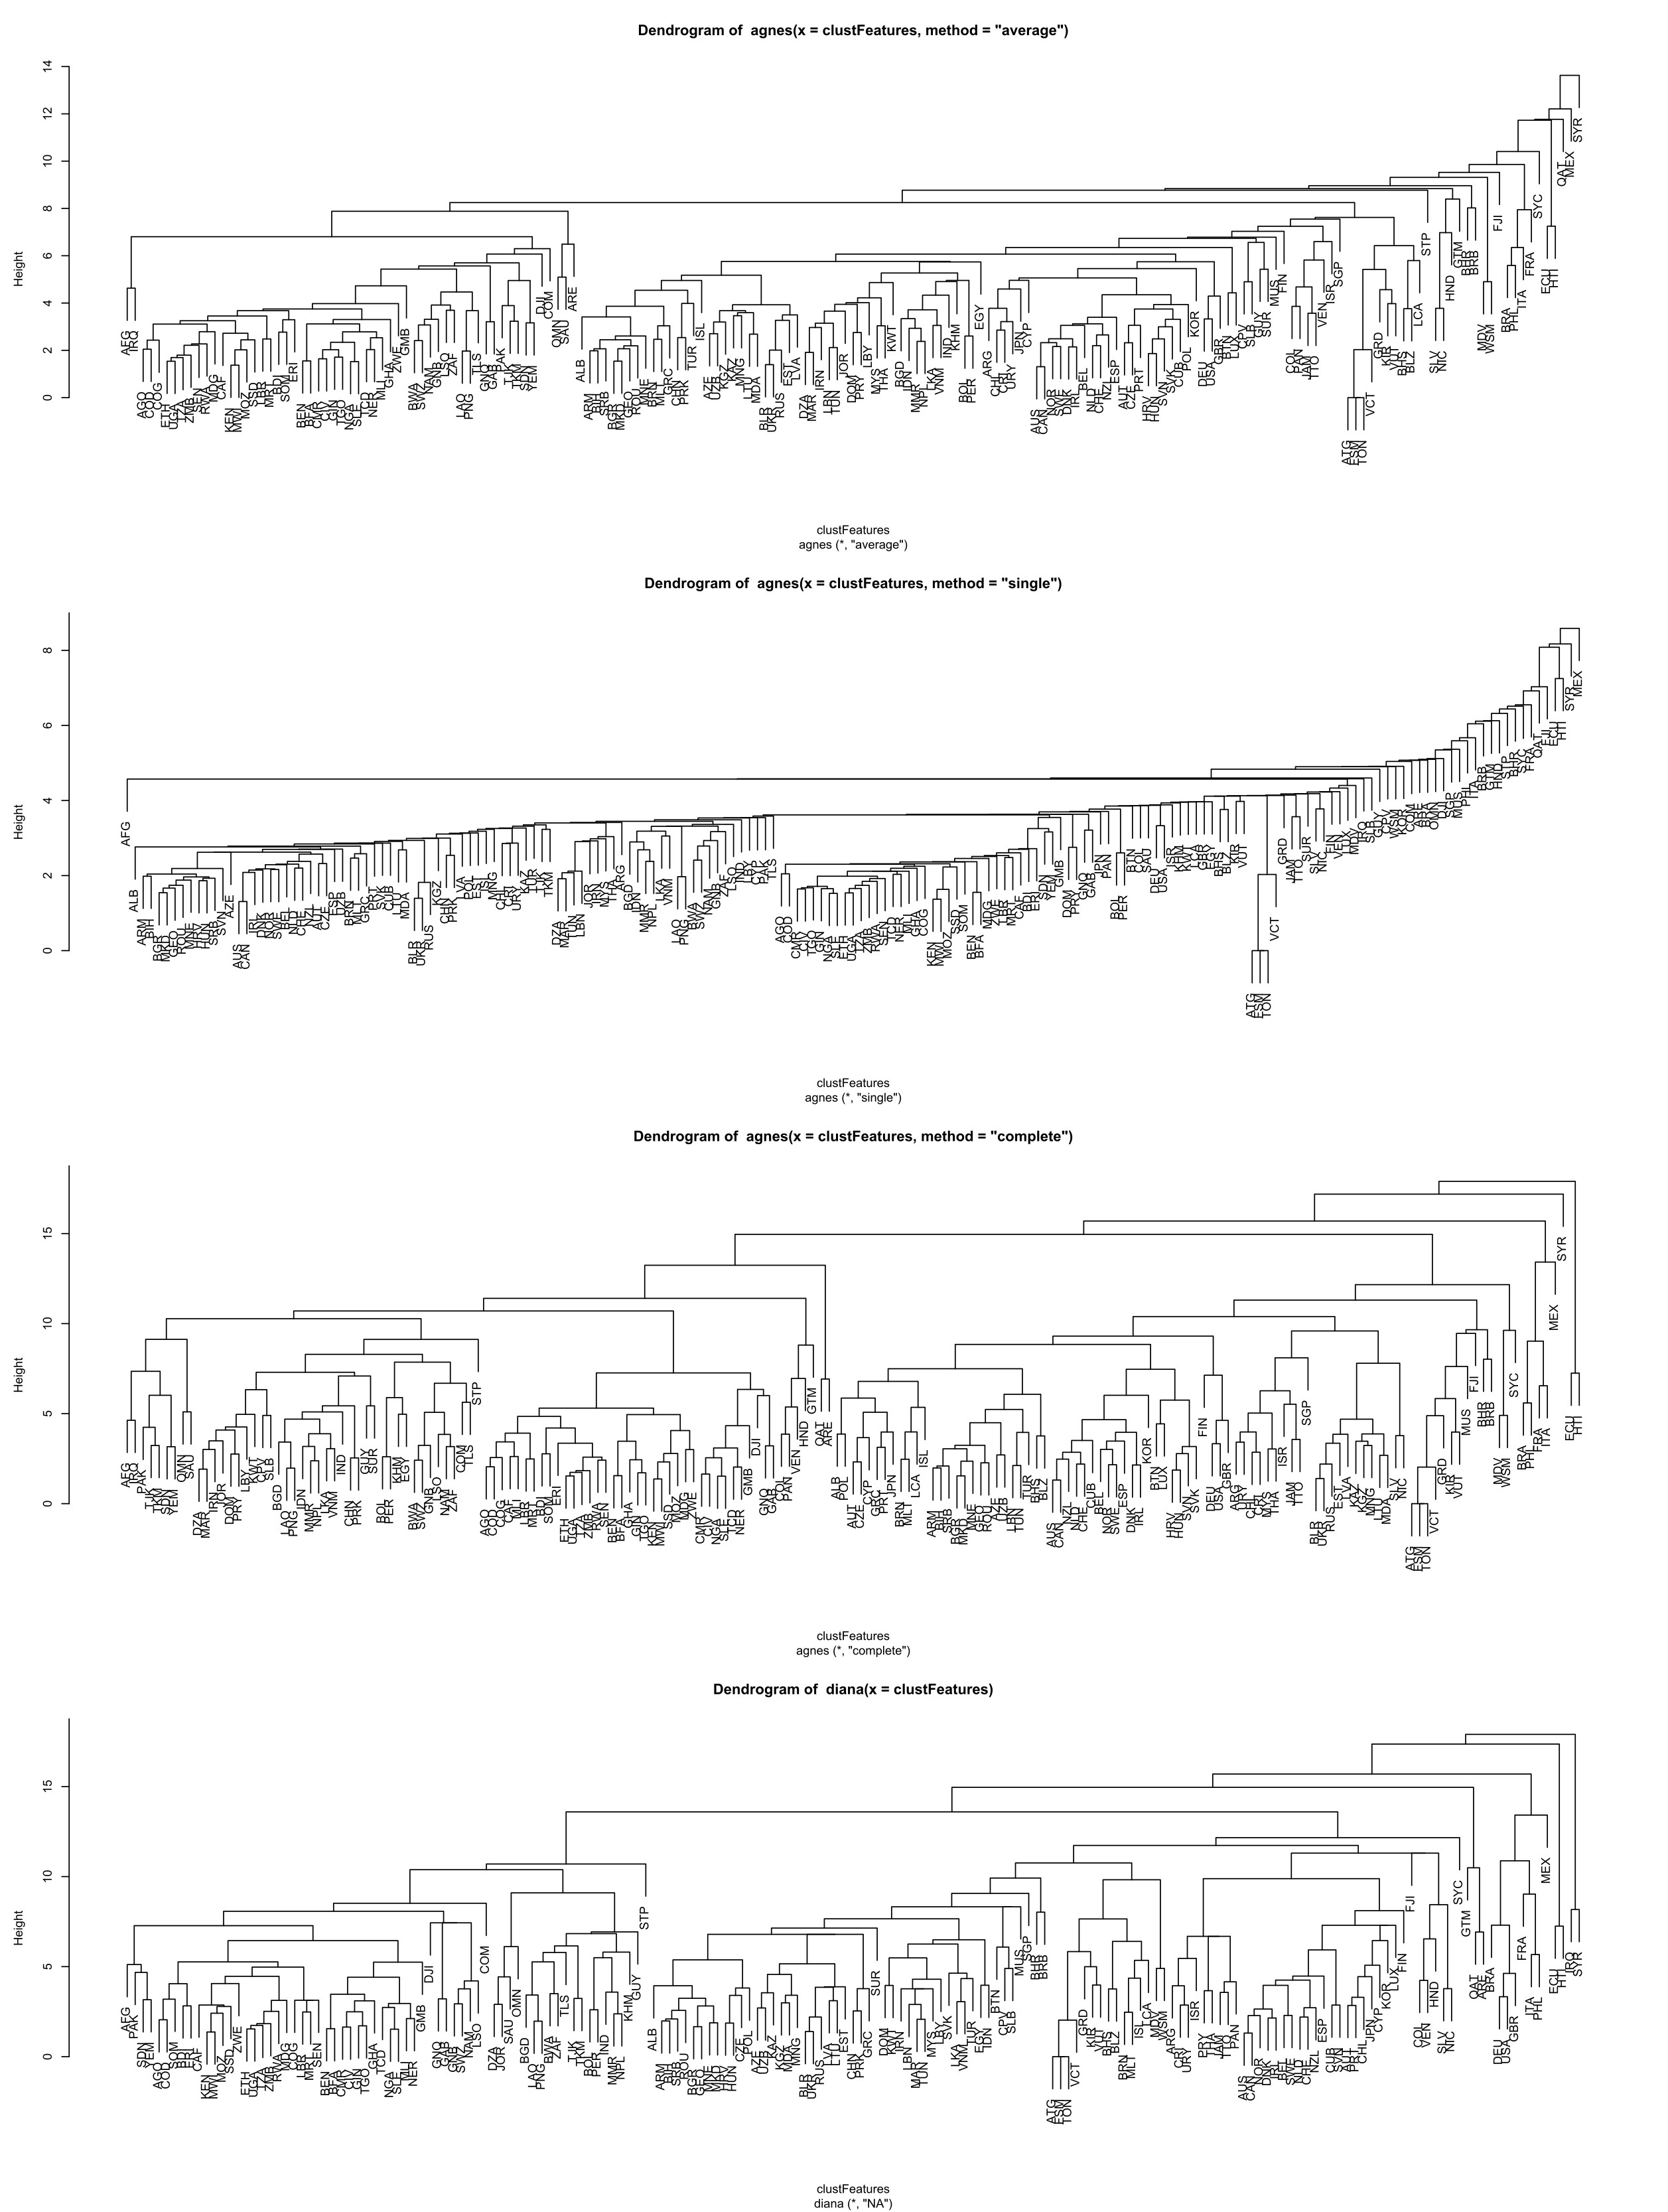
\includegraphics[height=\textheight]{figures/hierachicalClusteringScaledDendogram.jpg}
	\caption{Hierchical clustering dendograms met schalen}
	\label{fig:hcd}
\end{figure}
\begin{figure}
	\centering
	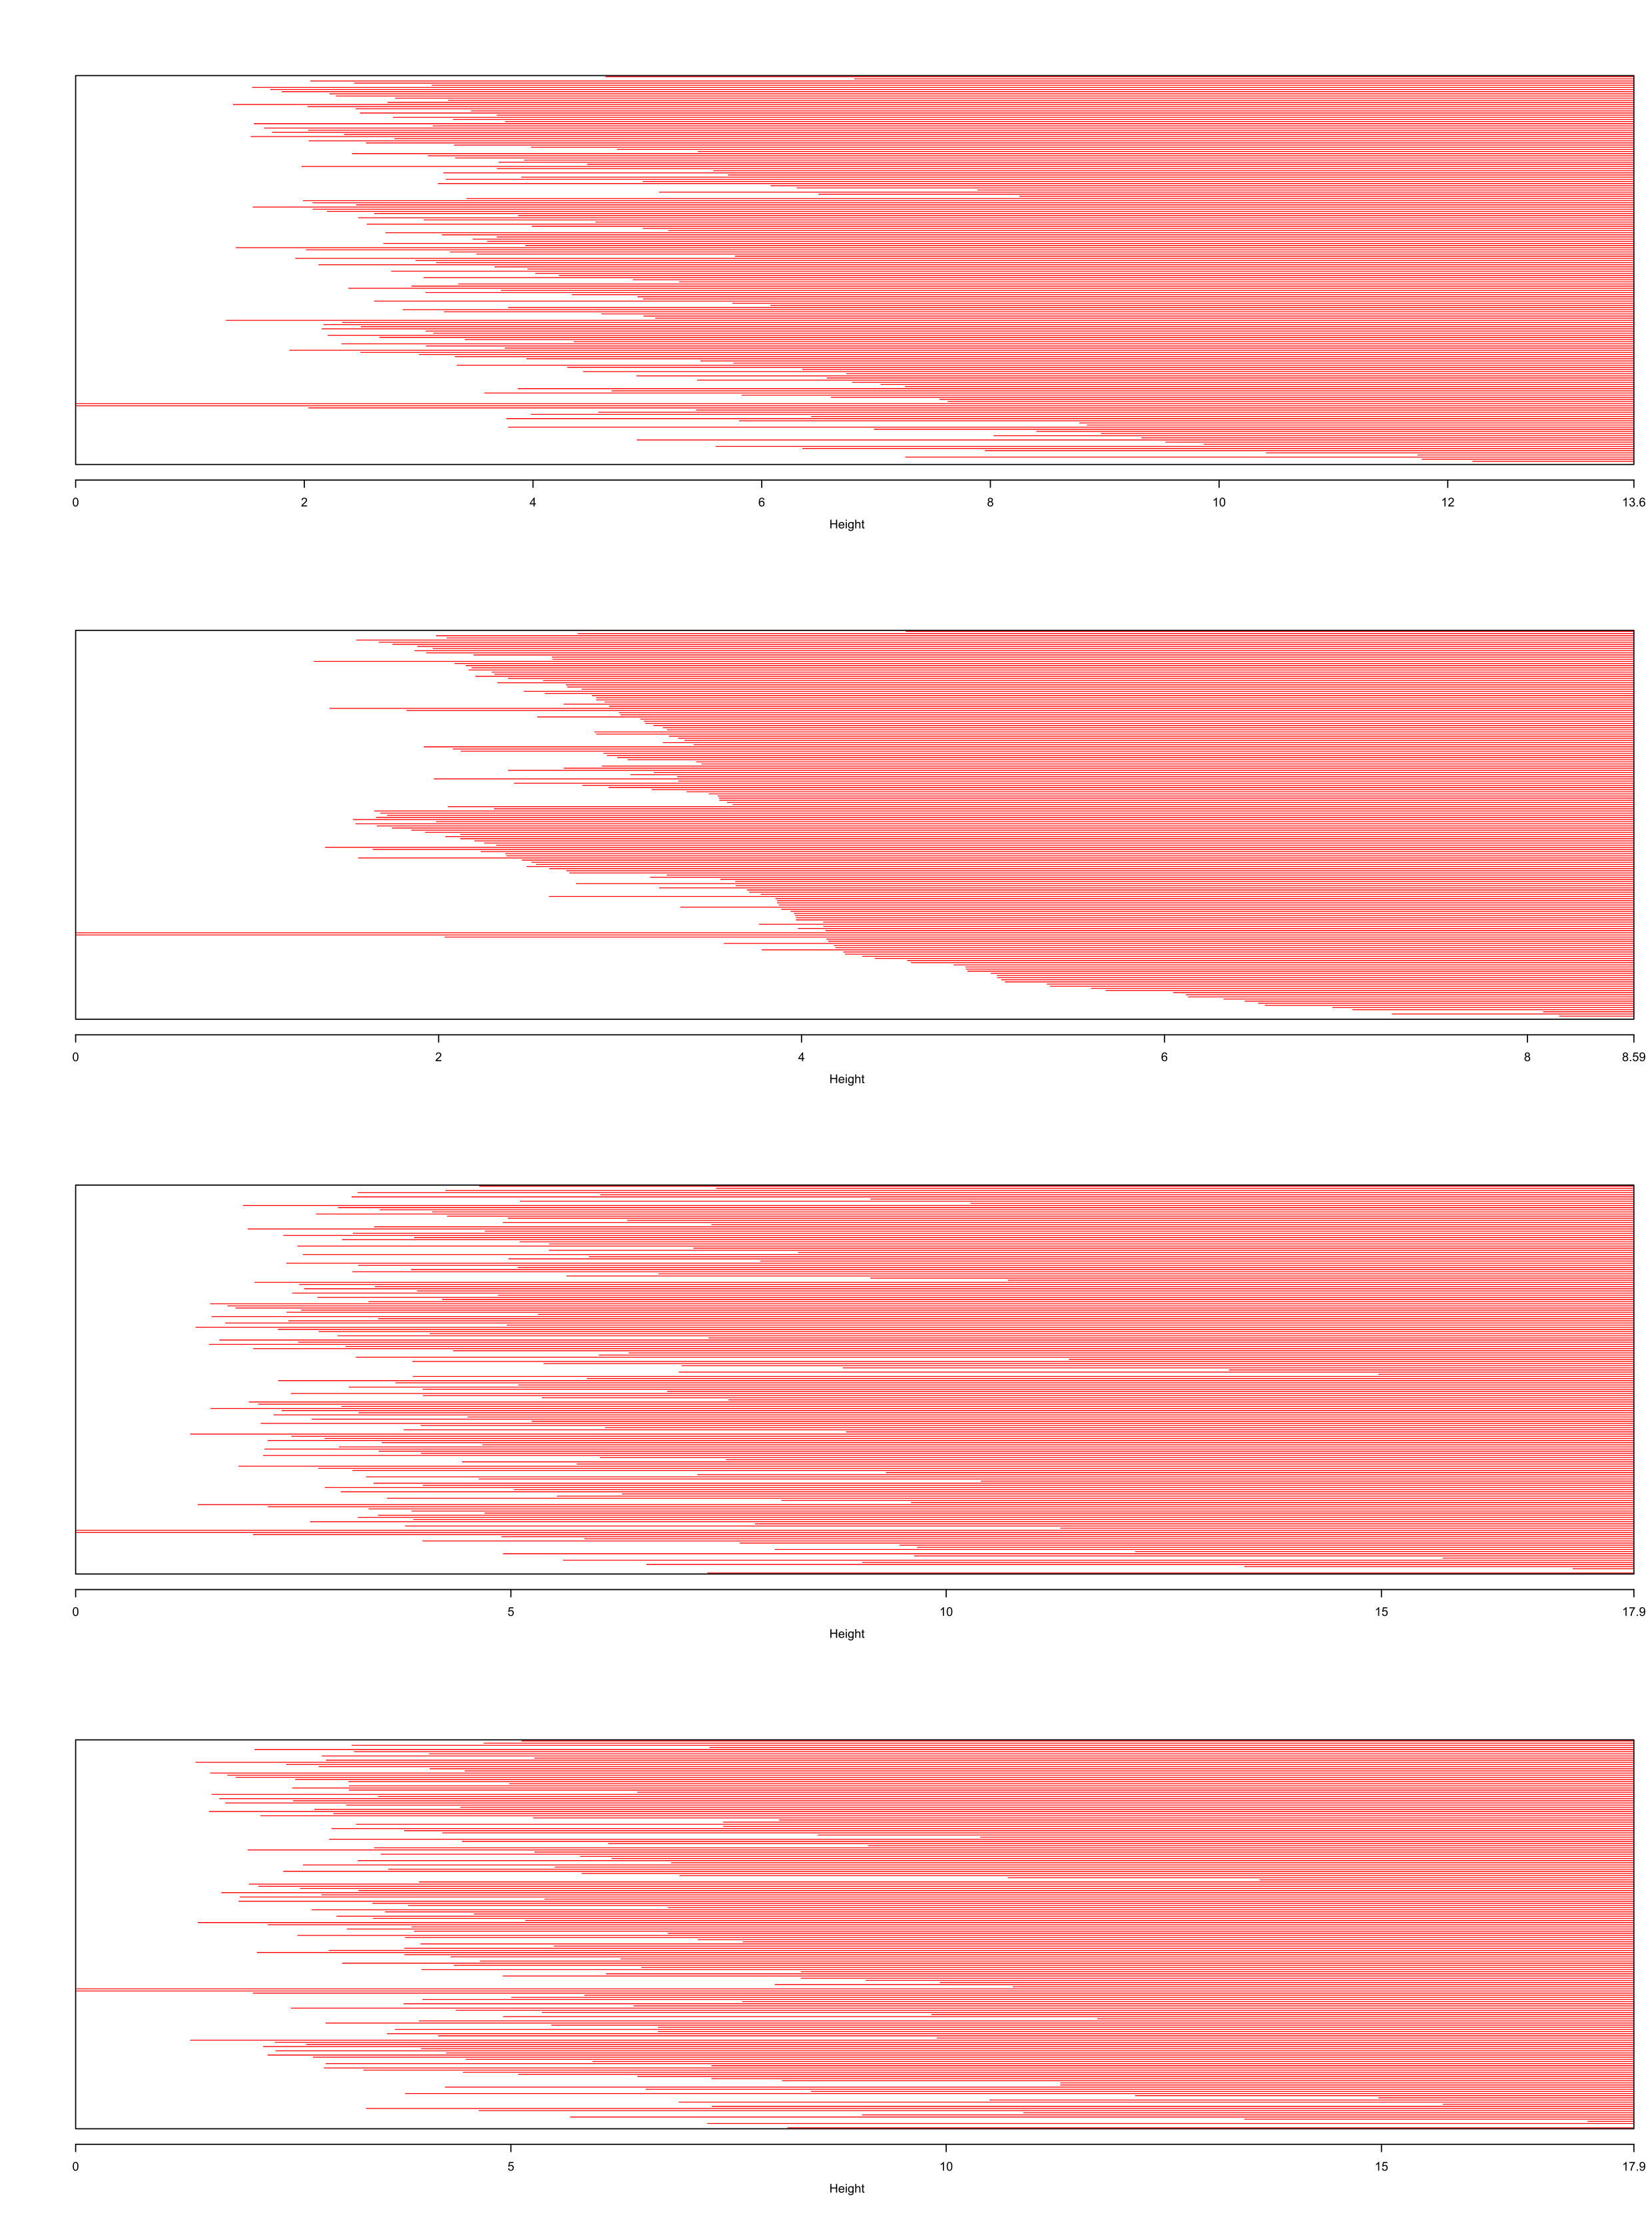
\includegraphics[height=\textheight]{figures/hierachicalClusteringScaledBanner.jpg}
	\caption{Hierchical clustering bannerplots met schalen}
	\label{fig:hcb}
\end{figure}
\begin{figure}
	\centering
	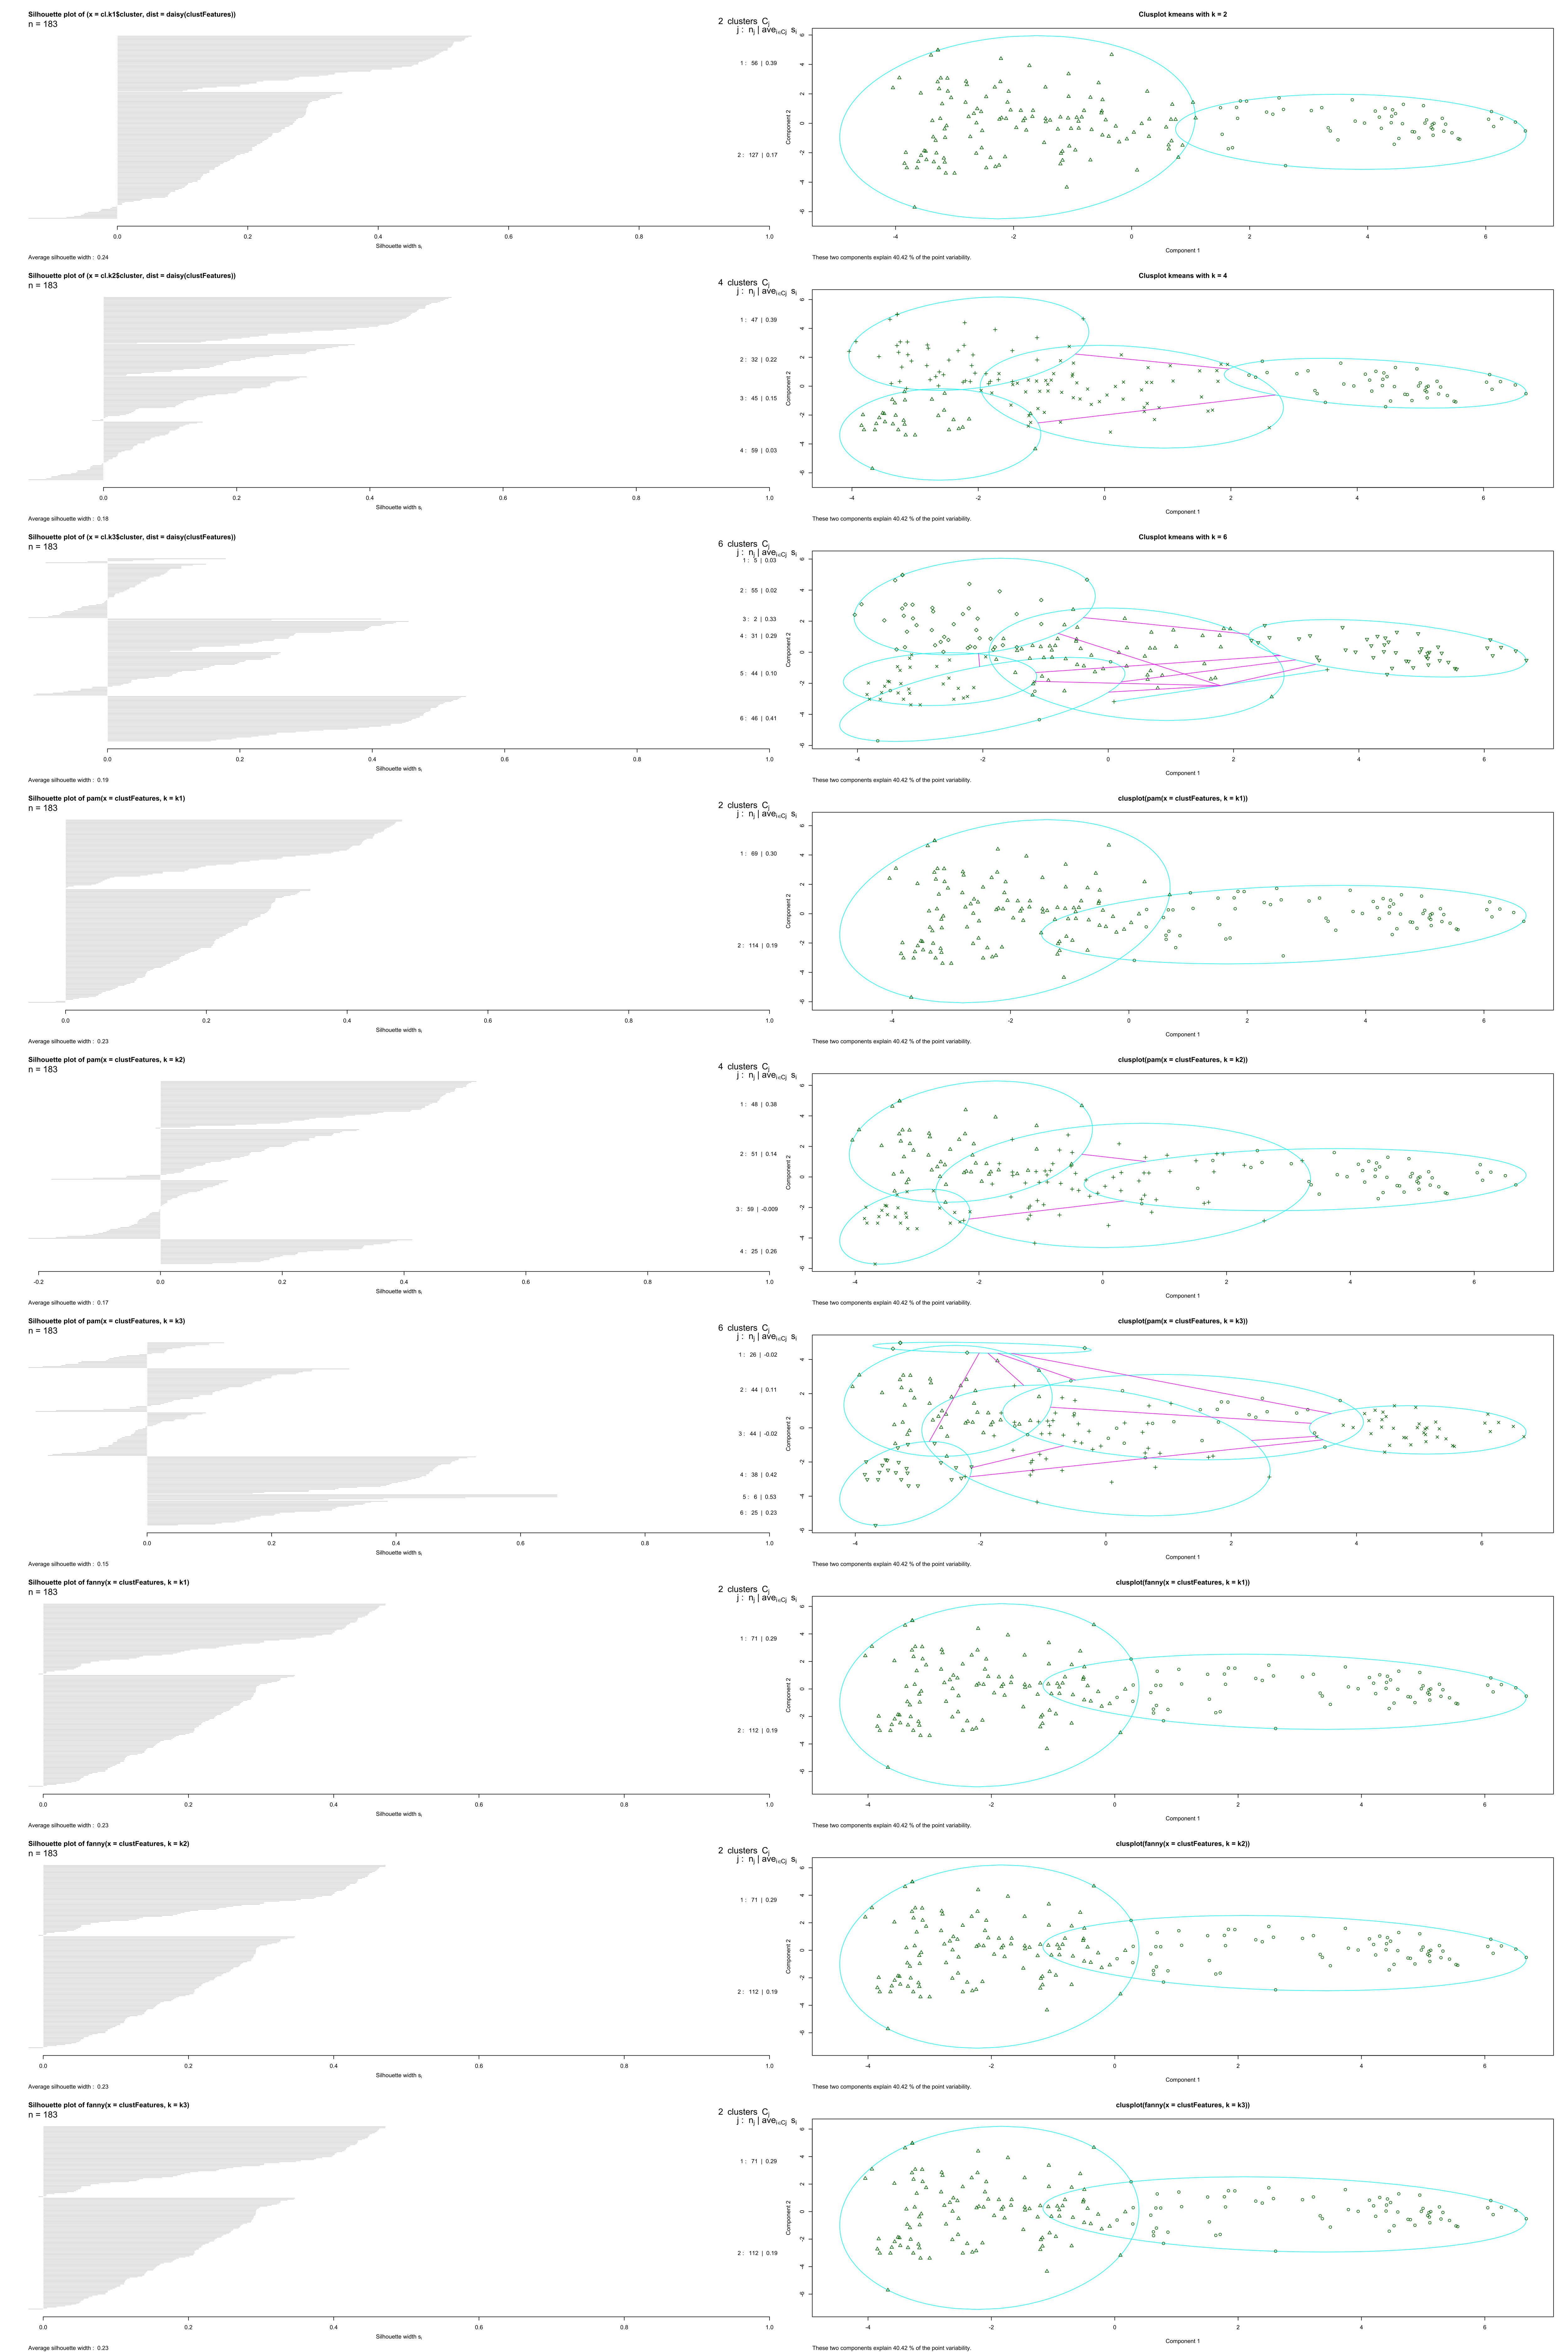
\includegraphics[height=\textheight]{figures/clusteringEvaluationScaled.jpg}
	\caption{Clustering evaluatie met schalen}
	\label{fig:ce}
\end{figure}


 
\end{document}
